\section{Fourier Theorie}
Die Fourier-Analysis wird vor allem verwendet um zeitliche Signale in ihre Frequnzanteile zu zerlegen. Aus der Summe dieser Frequenzanteile lässt sich das Signal wieder rekonstruieren.

\subsection{Trigonometrie ($z \in \mathbb{C})$}
\[\sin(z) = \frac{e^{jz} -e^{-jz}}{2j} \quad \cos(a) = \frac{e^{jz} +e^{-jz}}{2} \quad \tan(z) = \frac{\sin(z)}{\cos(z)}\]

\subsection{Testfunktion}
Sinus kann als Testfunktion von LTI-System verwendet werden, um Ausgangssignale zu rekonstruieren. Die Antwort eines LTI-Systems auf eine komplexe e-Funktion, ist wieder eine komplexe e-Funktion mit \textbf{derselben Kreisfrequenz} $\omega$ aber anderer Amplitude oder Phasenverschoben.
\begin{align*}
	\mathcal{L}\{e^{j\omega t}\} &= y_\omega(0) \cdot e^{j\omega t}\\
	\mathcal{L}\{\sin(\omega t)\} &= A(\omega) \cdot \sin(\omega t + \Phi(\omega))
\end{align*}

\subsection{Frequenzgang}
Der Frequenzgang $H(\omega)$ bestimmt die Änderung von Amplitude und Phase des Eingangssignals. In $\mathbb{R}$ wird die Funktion in \textbf{Amplitudengang} $\left|H(\omega)\right|$ und $\Phi(\omega)$ \textbf{Phasengang} zerlegt.
\begin{align*}
	A(\omega) &= \left|H(\omega)\right| = \sqrt{H(\omega) \cdot \overline{H(\omega)}} \\
	\Phi(\omega) &= \arg(H(\omega)) = \begin{cases*}
		\arccos\left(\frac{\Re(H(\omega))}{|H(\omega)|}\right) \qquad \text{für } \Im(H(\omega)) \geq 0 \\
		-\arccos\left(\frac{\Re(H(\omega))}{|H(\omega)|}\right) \qquad \text{für } \Im(H(\omega)) < 0
	\end{cases*}
\end{align*}
\textbf{Wichtig:} Siehe auch Laplace Übertragungsfunktion Kapitel \ref{ü-funktion}.


\noindent\textbf{Beispiel $\mathbb{C}$:} Frequenzgang von DGL $\ddot{u}(t) + \dot{u}(t) + u(t) = \sin(2t)$\\
\begin{align*}
	u(t) &= H(\omega)\cdot e^{j\omega t} \\
	\dot{u}(t) &= j\omega \cdot H(\omega)\cdot e^{j\omega t} \\
	\ddot{u}(t) &= \underbrace{j^2}_{-1}\omega^2 \cdot H(\omega)\cdot e^{j\omega t} 
\end{align*}
In DGL einsetzen und mit $e^{j\omega t}$ kürzen:
\begin{align*}
		 -\omega^2H(\omega) +  j\omega \cdot H(\omega)+H(\omega) = 1 \\
		 H(\omega) = \frac{1}{-\omega^2 + j\omega + 1}
\end{align*}

\noindent Mit $\sin(2t) = \frac{1}{2j}\left(e^{j2t} - e^{-j2t}\right)$ ergibt das im Komplexen ein $\omega = \pm2$ und reagiert mit $u(t) = H(\omega)\cdot\frac{1}{2j}(e^{j\omega t} - e^{-j\omega t})$. Die $\omega$ können nun in Frequenzgang $H(\omega)$ eingesetzt werden.
\[
H(2) = \frac{-3 -2j}{13}\qquad H(-2)= \frac{-3 + 2j}{13}
\]
Weil ein LTI-System vorliegt, können e-Funktionen einzeln mit Frequenzgang multipliziert werden.
\begin{align*}
	u(t) &= \frac{1}{2j}\left(H(2)\cdot e^{2jt} - H(-2)\cdot e^{-2jt}\right) \\
	&= \frac{1}{2j}\left(\frac{-3}{13}\cdot\frac{-2j}{13}\cdot e^{2jt} - \frac{-3}{13}\cdot\frac{2j}{13}\cdot e^{-2jt} \right) \\
	&= -\frac{3}{13}\cdot \underbrace{\frac{1}{2j}\left(\cdot e^{2jt} - e^{-2jt} \right)}_{\sin(2t)} - \frac{2}{13}\cdot \underbrace{\frac{1}{2}\left(\cdot e^{2jt} + e^{-2jt}\right)}_{\cos(2t)}  \\
	&= -\frac{3}{13}\sin(2t) - \frac{2}{13}\cos(2t)
\end{align*} 
\textbf{Hinweis:} Falls Parameter gefragt ist, Eingangssignal mit $H(\omega)$ multiplizieren und Parameter mit Ausgangssignal abgleichen.


\subsection{Fourier Transformation}
Fourier Transformation existiert für $F(\omega)$, wenn $f(t)$ absolut Integrierbar ist $\int\limits_{-\infty}^{\infty}|f(t)|dt < \infty$.
\begin{align*}
	F(\omega) &= \int_{-\infty}^{\infty}f(t)e^{-j \omega t}dt \\
	f(t) &= \frac{1}{2\pi}\int_{-\infty}^{\infty}F(\omega)e^{j \omega t}d\omega
\end{align*}

\subsection{Eigenschaften}
Siehe Fourier-Tabelle

\subsection{Korrespondenzpaar}
Falls ein Korrespondenz $K$ gegeben ist, kann dies mittels Umformung Transformiert werden\\
\noindent\textbf{Beispiel} $K := e^{-at^2} \transform \sqrt{\frac{\pi}{a}}e^{-\frac{\omega^2}{4a}}$ damit lässt sich $a = 3$ bestimmen. 
\begin{align*}
	g(t) &= e^{-3t^2 + 12t - 11} = e^{-3(t^2 -4t + 4) + 1} = e\cdot e^{-\overbrace{3}^{a}(\overbrace{t-2}^{\text{Verschiebung}})^2}\\
	G(\omega) &= e\cdot e^{-2j\omega}\sqrt{\frac{\pi}{3}}e^{-\frac{\omega^2}{12}} = \sqrt{\frac{\pi}{3}}e^{1-\frac{\omega^2}{12}-2j\omega}
\end{align*}

\subsection{DFT}
Die Diskrete Fourier Transformation ist die Grundlage für viele digitale Processe wie Kompressionen etc. Dabei ist $k$ der Index von $c_k$.
\begin{align*}
	x[n] &= \sum_{k=0}^{N-1}c_k e^{jk(2\pi/N)n}  \\
	c_k &= \frac{1}{N}\sum_{n=0}^{N-1}x[n]e^{-jk(2\pi/N)n}
\end{align*}


\subsection{Amplituden- und Phasendichte}
\todo{
	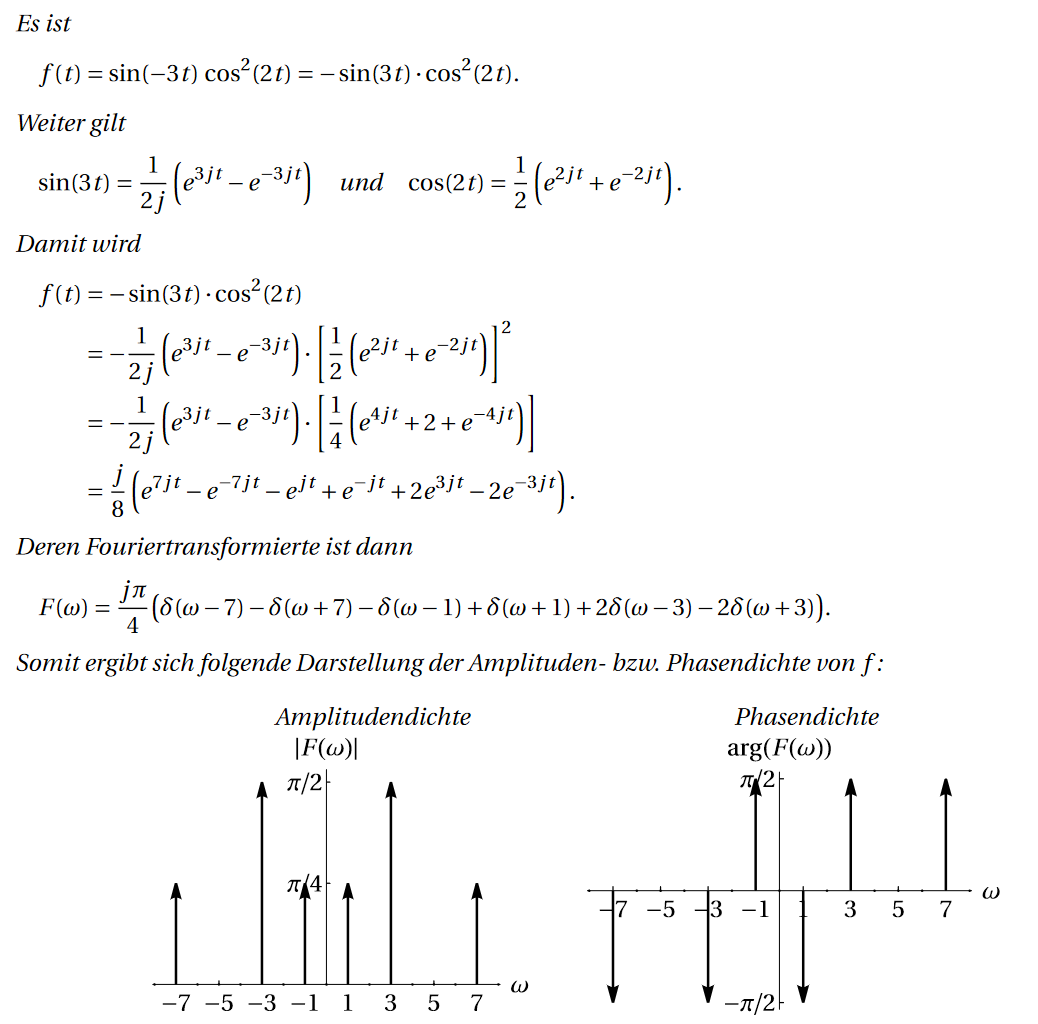
\includegraphics[width=\columnwidth]{Images/screenshot001}
}